%%%%%%%%%%%% BEGIN PREAMBLE 
\documentclass[aspectratio=169, serif]{beamer}
%\usepackage[T1]{fontenc}
\usepackage[utf8]{inputenc}
\usepackage{biolinum}
\usepackage{mathtools}
\setbeamertemplate{bibliography item}[text]
\usepackage{microtype}
\usepackage{bm}
\usepackage{amssymb}
\usepackage{wasysym}
\usepackage{mathrsfs}
\usepackage{setspace,tikz,xcolor,listings,multicol}
\usepackage{ragged2e}
\usetikzlibrary{arrows,matrix}
\usepackage[vcentermath]{youngtab}
\usepackage[english]{babel}
\usepackage[utf8]{inputenc}
\usepackage{tcolorbox}
\usepackage{xcolor}
\newcommand{\arxiv}[1]{\href{http://arxiv.org/abs/#1}{\texttt{arXiv:#1}}}
\definecolor{pink}{RGB}{24, 117, 18}
\definecolor{purple}{RGB}{102, 27, 194}
\definecolor{red}{RGB}{235, 7, 90}
\definecolor{yellow}{RGB}{255, 170, 0}
\newcommand{\ph}{\phantom{.}}
\definecolor{forGreen}{RGB}{0,120,0}
\definecolor{skyBlue}{RGB}{0, 200, 255}
\newcommand{\fgcf}{\scriptsize\color{forGreen}4}
\newcommand{\fgct}{\scriptsize \color{forGreen}2}
\newcommand{\tn}{10}
\DeclareMathOperator{\SD}{SD}
\DeclareMathOperator{\Pt}{P}
\DeclareMathOperator{\sh}{sh}

\usepackage{mathtools}
\usepackage{ytableau}
\usepackage[all]{xy}
\usefonttheme{serif}
\usetheme[nofirafonts]{focus}
\setbeamertemplate{frametitle continuation}{}
\setbeamertemplate{caption}[numbered]
\definecolor{main}{RGB}{0, 75, 135}
\newcommand{\switchyarrowy}{\mathrlap{\curvearrowleft}\hspace{0.09em}\curvearrowright}
\renewcommand{\thempfootnote}{\arabic{mpfootnote}}
\title{The Box-Ball System}
\institute{\vspace{-2em}UConn REU}
\date{\vspace{-2em}July 24, 2020}
\begin{document}
\begin{frame}
    \maketitle
      \centering
  \begin{tabular}{c c c c}
  
    
\includegraphics[width=.1\linewidth]{Ben.jpeg} &     
\includegraphics[width=.1\linewidth]{Eli.jpeg}  & 
\includegraphics[width=.1\linewidth]{Aubrey.jpeg}  &
    
\includegraphics[width=.1\linewidth]{Rose.jpeg} \\
    
    \textbf{Ben Drucker} & \textbf{Eli Garcia} & \textbf{Aubrey Rumbolt} & Rose Silver \\
    \end{tabular}
    
    \centering
\end{frame}
\begin{frame}{Overview}
    \begin{enumerate}
        \item Introduction: permutations, tableaux, Knuth relations, and the RSK algorithm
        \item The box-ball system
        \item Results and conjectures: steady state times and soliton decompositions
    \end{enumerate}
\end{frame}
\section{Introduction}
\begin{frame}{Permutations}
\begin{block}{Definition. (Permutation)}
A permutation $\pi$ of $n$ numbers is a bijective function from the set of natural numbers $\{1,2,...,n\}$ to itself.
Let $S_n$ be the set of all possible permutations of $n$ numbers.
\end{block}
\begin{exampleblock}{Example. (Permutation)}
In $S_6$, a permutation $\sigma$ may consist of the following mappings:
\begin{align*}
1&\mapsto 3\\[-.5em]
2&\mapsto 4\\[-.5em]
3&\mapsto 2\\[-.5em]
4&\mapsto 1\\[-.5em]
5&\mapsto 5\\[-.5em]
6&\mapsto 6
\end{align*}
\end{exampleblock}
\end{frame}
\begin{frame}{Permutations: Notation}
\small
    \begin{exampleblock}{Example. (2-line Notation)} We may write permutations compactly using 2-line notation. For example, in 2-line notation,
    \centering
$\sigma = \begin{pmatrix}1&2&3&4&5&6\\3&4&2&1&5&6\end{pmatrix}\begin{matrix*}[l]{\color{forGreen} \leftarrow\text{(1 through n)}}\\ {\color{forGreen}\leftarrow \text{(mappings)}} \end{matrix*}$
\end{exampleblock}
\begin{exampleblock}{Example. (1-line Notation)}
We may write permutations even more compactly using 1-line notation. For example, in 1-line notation, $\sigma = 342156{\color{forGreen}~\leftarrow\text{ (just mappings)}}.$
\end{exampleblock}
\begin{block}{Note.}
From now on, we will use the 1-line notation whenever permutations are used.
\end{block}
\end{frame}
\begin{frame}{Knuth Relations}
    \begin{definition}
        Suppose $\pi$, $\sigma \in S_n$ and $x<y<z$.
            \begin{itemize}
                \item $\pi$ and $\sigma$ differ by a Knuth relation of the \textbf{first kind} ($K_1$) if \begin{center} $\pi=x_1...\textcolor{purple}{y}\textcolor{red}{x}\textcolor{pink}{z}...x_n$ and $\sigma=x_1...\textcolor{purple}{y}\textcolor{pink}{z}\textcolor{red}{x}...x_n$ \end{center} 
                
                \item $\pi$ and $\sigma$ differ by a Knuth relation of the \textbf{second kind} ($K_2$) if \begin{center} $\pi=x_1...\textcolor{red}{x}\textcolor{pink}{z}\textcolor{purple}{y}...x_n$ and $\sigma=x_1...\textcolor{pink}{z}\textcolor{red}{x}\textcolor{purple}{y}...x_n$ \end{center}  
                
                \item $\pi$ and $\sigma$ differ by Knuth relations of \textbf{both kinds} ($K_B$) if for $x<y_1<z$ and  $x<y_2<z$\begin{center} $\pi=x_1...\textcolor{yellow}{y_1}\textcolor{red}{x}\textcolor{pink}{z}\textcolor{purple}{y_2}...x_n$ and $\sigma=x_1...\textcolor{yellow}{y_1}\textcolor{pink}{z}\textcolor{red}{x}\textcolor{purple}{y_2}...x_n$ \end{center}
            \end{itemize}
    \end{definition}
\end{frame}
\begin{frame}{Tableaux}
    \begin{block}{Definition. (Young Tableaux)}
        \begin{itemize}
        \small
            \item A Young tableau (pl. tableaux) is an arrangement of numbers $\{1,2,...,n\}$ into rows whose lengths are weakly decreasing.\vspace{-0.25em}
            \item The Young tableau is \textit{standard} if each row is an increasing sequence (going from left to right) and each column is an increasing sequence (going from top to bottom). \vspace{-0.25em}
            % A Young tableau is \textit{nonstandard} if this is not the case.
            \item The \textit{reading word} of a standard Young tableau is the permutation formed by concatenating the rows of the tableau from bottom to top.
        \end{itemize}
    \end{block}
    \begin{exampleblock}{Example. (Standard Young Tableau)}
        \begin{itemize}
        \item \raisebox{-1em}{\tiny \young(12,34,5)} is a standard Young tableau. Its reading word is $53412.$ %PERM: [3, 1, 5, 4, 2]
        \item \raisebox{-1em}{\tiny \young(12,4,5,3)} is a nonstandard Young tableau.
        \end{itemize}
        \vspace{-3.8pt}
    \end{exampleblock}
\end{frame}
\begin{frame}{Robinson-Schensted-Knuth insertion algorithm}
        \begin{center}
            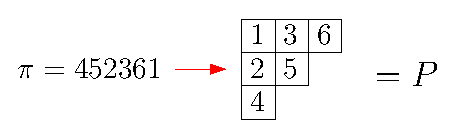
\includegraphics[scale = 0.85]{RS_Example.eps}
        \end{center}
    Let $P$ be the empty tableau. Given a permutation $\pi = \pi_1\cdots\pi_n,$ the \textit{Robinson-Schensted-Knuth (RSK) insertion algorithm} is a method of insertion of each element of $\pi$ into $P.$ The RSK insertion algorithm ensures that the result---after all elements of $\pi$ have been inserted---will be a standard Young tableau.
\end{frame}
\section{The Box-Ball System}
\begin{frame}{Box-Ball System}
        Consider an initial configuration $\pi=\pi_1\pi_2\pi_3...\pi_k$, where $\pi$ is a permutation in 1-line notation.
        \vspace{5mm}
        \newline To complete a box-ball move, we let each number (or ``ball'') jump to the next available spot (or ``box'') to the right. We first move 1, then we move 2, and so on.
        
    \end{frame}

    \begin{frame}{Box-Ball System: Example---$\pi=452361$}
    \centering
        We will use the example permutation $\pi=452361$.\\
        \pause
        \RaggedRight
        \vspace{2mm}
        \boxed{\text{\textit{Step 1:}}}\phantom{---}Write the permutation on a strip of infinite boxes as shown below.\\\centering This configuration corresponds $t=0$.\\
        \RaggedRight
        \begin{figure}[H]
            \centering
            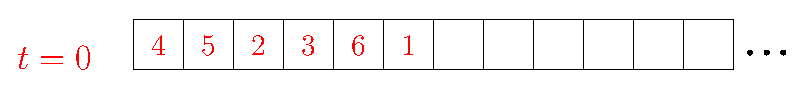
\includegraphics[width = 5in]{Step_1.eps}
        \end{figure}
        \pause
        \boxed{\text{\textit{Step 2:}}}\phantom{---}Going from smallest to largest, move each number to the next empty box to the right.\\
        \begin{figure}[H]
            \centering
            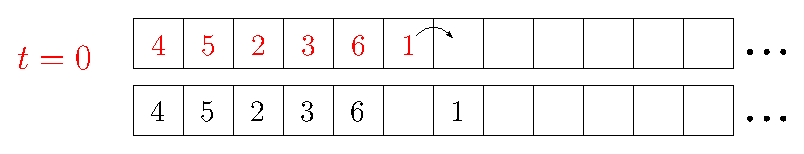
\includegraphics[width = 5in]{Step2V2.eps}
        \end{figure}    
    \end{frame}
    \begin{frame}{Box-Ball System: Example---$\pi=452361$}
        \boxed{\text{\textit{Step 3:}}}\phantom{---}Continue moving numbers from smallest to largest to their nearest available spots until every number in the permutation has been moved. We are now at the $t=1$ state and we have completed one BBS move.
        \pause
        \begin{figure}
            \centering
                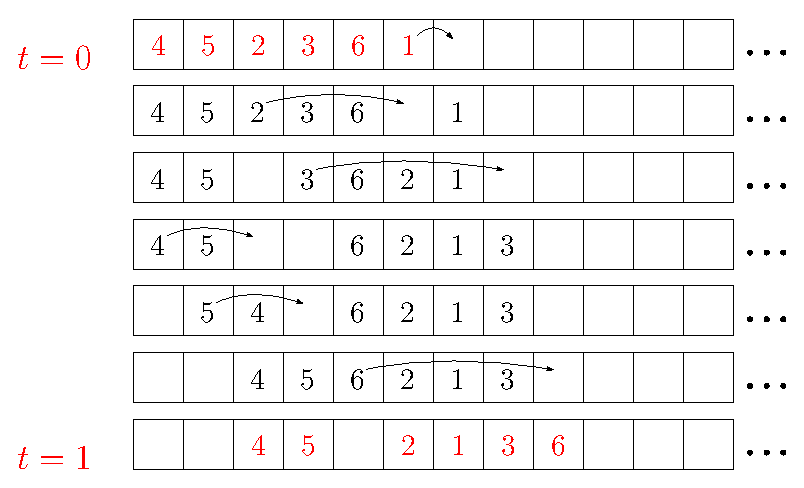
\includegraphics[width = 3.2in]{Step3.eps}
        \end{figure}
    \end{frame}
    \begin{frame}{Box-Ball System: Example---$\pi=452361$}
        \boxed{\text{\textit{Step 4:}}}\phantom{---}Continue making BBS moves.\\
        \phantom{\boxed{Step 4:}---}(Here, 4 moves are shown).
        \begin{figure}
            \centering
            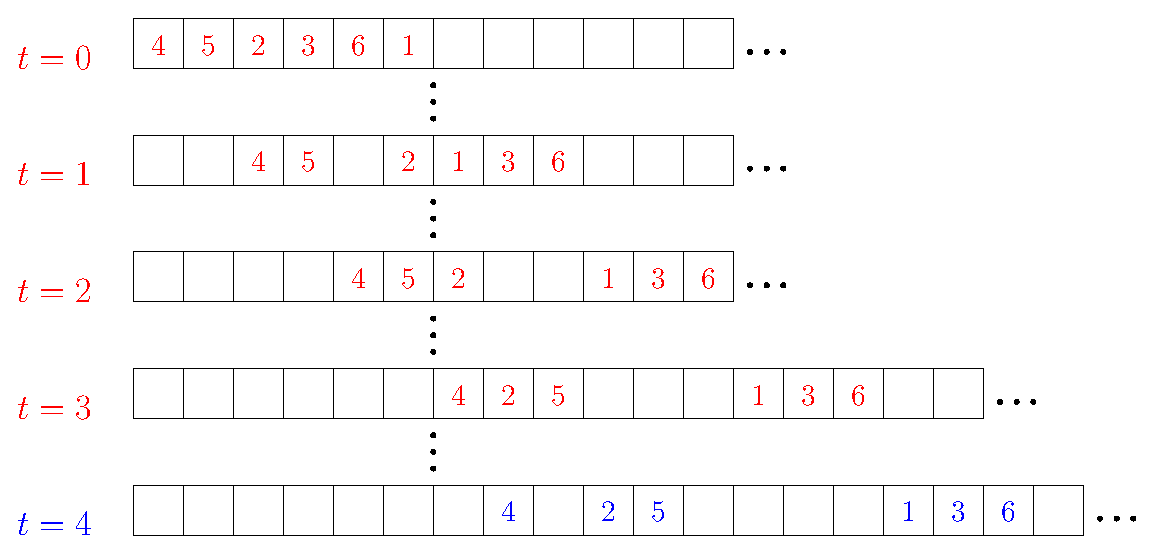
\includegraphics[width = 2.85in]{Step4V2.eps}
            \end{figure}
    \pause
    \begin{block}{Note. (Backwards BBS)}
    \begin{itemize}
    \small
        \item We now move balls from \textbf{largest-to-smallest} to their nearest available spaces to the \textbf{left}.
        \item The time-values after each backwards box-ball move now \textbf{decrease}. 
        %\item We denote the soliton decomposition of this system the \textbf{``backwards soliton decomposition''} of a permutation.
    \end{itemize}
    \end{block}
\end{frame}
\iffalse
\begin{frame}{Box-Ball System: Backwards BBS}
    \begin{exampleblock}{Example. (Backwards BBS)}
    \centering
    \begin{tabular}{c|cccccccccccccc}
         $t = 0$& $e$&$e$&$e$&$e$&$e$&$e$&$e$&$e$&3&2&4&1&5&6 \\
         $t = -1$& $e$&$e$&$e$&$e$&3&4&5&6&2&$e$&1&$e$&$e$&$e$ \\
         $t = -2$&3&4&5&6&$e$&$e$&$e$&2&$e$&1&$e$&$e$&$e$&$e$
    \end{tabular}
    \end{exampleblock}
\end{frame}
\fi
\iffalse
    \begin{frame}{Partitions}
\begin{block}{Definition. (Partition)}
A partition of a non-negative integer $n$ is a sequence $(p_1, p_2, ..., p_\ell)$ such that $\sum_{i=1}^\ell p_i = n,$ with $p_1 \geq p_2 \geq ...\geq p_\ell$. Partitions are equivalent if their nonzero elements are equal and placed identically. Typically, zero-entries are not written.
\end{block}
\begin{exampleblock}{Example. (Partition)}
    $(4,4,2,0,0,0) = (4,4,2)$ is a partition of 10 since $4+4+2=10$ and $4\geq 4\geq 2$.
\end{exampleblock}
\begin{exampleblock}{Example. (Young Diagram)}
    We may represent the partition above using the following diagram.\\
    \centering
    \young(\ph\ph\ph\ph,\ph\ph\ph\ph,\ph\ph) \raisebox{1.35em}{\color{forGreen} \begin{tabular}{c}
         $\leftarrow 4$\\
         $\leftarrow 4$\\
         $\leftarrow 2$
    \end{tabular}}
\end{exampleblock}
\end{frame}
\fi
     \begin{frame}{Box-Ball System: Soliton Decomposition}
        At a certain point, the system reaches a \emph{steady state} where:
        \begin{itemize}
            \item blocks of increasing sequences (or \emph{solitons}) move together at a speed equal to their length.
            \item the sizes of the solitons are weakly increasing from left to right
            \item order of the solitons remain unchanged
        \end{itemize}
       
        \begin{figure}
            \centering
            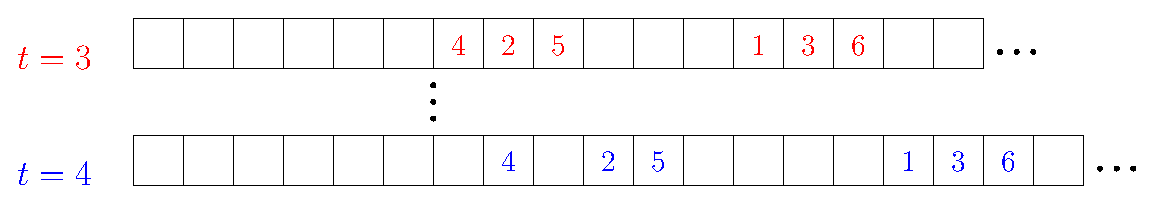
\includegraphics[width = 4in]{ExtraEPS.eps}
        \end{figure}
        
    \end{frame}

    \begin{frame}{Box-Ball System: Example---$\pi=452361$}
        \boxed{\text{\textit{Step 5:}}}\phantom{---}After reaching steady state, create a diagram by stacking solitons from right to left. The shape of the diagram forms a (not necessarily standard) Young tableau:\\
        \begin{figure}
            \centering
            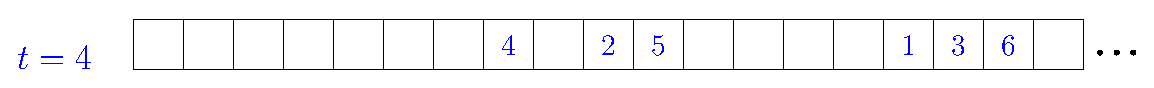
\includegraphics[width = 5in]{Step5.eps}
        \end{figure}
        \begin{figure}
            \centering
            Soliton decomposition
            ~
            %shape 
            %= 
            $\young(136,25,4)$  with shape $(3,2,1)$.
        \end{figure}
    \begin{block}{Central Questions.}
    When is soliton decomposition standard? When is soliton decomposition equal to the original permutation's $P$-tableau? How long does it take for a given permutation to reach its steady-state?
    \end{block}
    \end{frame}

\iffalse
\begin{frame}{Computational Infrastructure}
    \begin{itemize}
        \item The RSK-insertion algorithm
        \begin{itemize}
            \item The RS-partition ($\lambda$ and $\mu$) for a permutation
            \color{blue}
            \item The Localized RS-partition ($\lambda^L$ and $\mu^L$) for a permutation
        \end{itemize}
        \color{blue}
        \item Simulation of the box-ball system
        \begin{itemize}
            \color{blue}
            \item Systematic computation of the steady-state times of a ``large set" (e.g. $S_n$) of permutations
        \end{itemize}
        \item Knuth Moves
            \begin{itemize}
                \color{blue}
                \item Systematic computation of Knuth set partitions
                \item Graphing of said partitions with or without a poset structure
            \end{itemize}
    \end{itemize}
    \pause
    \begin{block}{High Performance Computing (hpc)}
        We have implemented multi-core processing in some of our programs and used UCONN's hpc cluster to speed up computation.
    \end{block}
\end{frame}
\fi
\section{Results and Conjectures}
\begin{frame}{Results Involving Soliton decomposition}
    \begin{itemize}
        \item The remainder of the presentation will focus on results and conjectures about the \emph{soliton decomposition} of a permutation, which we denote $\SD(\pi).$
    \end{itemize}
    \begin{block}{Big question (from earlier)}
        For what permutations $\pi$ do we have $\SD(\pi)=\Pt(\pi)$?
    \end{block}
\end{frame}
% \begin{frame}{Pattern avoidance}
%     \begin{itemize}
%         \item An interesting angle to approach this question from is \emph{pattern avoidance}.
%     \end{itemize}
%     \begin{block}{Conjecture}
%         If $\pi\in S_n$ avoids both $2143$ and $3142,$ then $\SD(\pi)=\Pt(\pi).$
%     \end{block}
%     \begin{block}{Conjecture}
%         If $\SD(\pi)\neq\Pt(\pi),$ then the reading word of $\Pt(\pi)$ contains \emph{consecutive} terms $``b_1acb_2"$ or $``b_1cab_2"$ where $a<b_1,b_2<c.$
%     \end{block}
% \end{frame}
\begin{frame}{Reformulating the question}
    \begin{itemize}
        \item A way to simplify (and answer) the big question is by formulating equivalent statements.
    \end{itemize}
    
     \begin{alertblock}{Theorem}
        The following are equivalent: \begin{enumerate}
            \item $\SD(\pi) = \Pt(\pi).$
            \item $\SD(\pi)$ is a standard tableau.
        \end{enumerate}
    \end{alertblock}
    \begin{block}{Conjecture}
        The following is equivalent to (1) and (2).
        \begin{enumerate}
            \setcounter{enumi}{2}
            \item $\sh\SD(\pi) = \sh\Pt(\pi).$ 
        \end{enumerate}
    \end{block}
    \begin{itemize}
        \item We have shown $(1)\Longleftrightarrow(2)$ and $(1) \implies (3).$ It remains to prove $(3)\implies(1).$
    \end{itemize}
\end{frame}
\begin{frame}{Knuth move perspective}
    \begin{itemize}
            \item Yet another way of attacking this problem is from the perspective of Knuth moves\footnote[frame]{The theorem on this slide is due in part to a result in \cite{LLPS19}.}
            \item Let $r$ denote the reading word of $P(\pi).$ The RSK theory tells us there is a path of Knuth moves from $\pi$ to $r.$
        \end{itemize}
        \begin{alertblock}{Theorems}
        \begin{itemize}
            \item If there exists a path from $\pi$ to $r$ such that no move along the path is $K_B,$ then $\sh\SD(\pi)=\sh P(\pi).$
            \item If there exists a path from $\pi$ to $r$ containing an odd number of $K_B$ moves, then $\SD(\pi)\neq P(\pi).$
        \end{itemize}
    \end{alertblock}
        % ALERT results
    
\end{frame}
\begin{frame}{Results Involving Steady-State Times}
    \begin{alertblock}{Theorem: Classification of permutations with steady-state value of $t=0$}
    A permutation $r$ has a box-ball steady-state value of $t=0$ if and only if $r$ is the reading word of a standard tableau.
    \end{alertblock}
    \begin{alertblock}{Theorem: Some permutations with steady-state value of $t=1$}
     Let $r$ be the reading word of a standard tableau $P$. If $K$ represents the action of a $K_1$ or $K_2$ move (but not $K_B$), then $r'=K(r)$ has a box-ball steady-state value of $t=1.$
    \end{alertblock}
    \small
    \begin{block}{$n-3$ conjecture}
        The steady-state time for a permutation in $S_n$ is no more than $n-3.$
    \end{block}
\end{frame}
%\begin{frame}{Results Involving Steady-State Times}
%    \begin{block}{An extension of the box-ball system.}
%    We may define a system very similar to the standard box-ball system we have previously defined called the ``backwards box-ball system." Instead of moving balls from smallest-to-largest to their nearest available spaces to the right, \textbf{we now move balls from largest-to-smallest to their nearest available spaces to the left. Also, the time-values after each backwards box-ball move decrease.} We denote the solition decomposition of this system the ``backwards soliton decomposition" of a permutation.
%    \end{block}
%\end{frame}
    %\begin{frame}{Results Involving Steady-State Times}
    %\begin{block}{Backwards permutation theorem}
    %Let $\pi,\sigma\in S_n.$ If $\sigma$ is a permutation formed by a backwards box-ball move of $\pi$ at some negative time, then $\sigma$ and $\pi$ have the same backwards soliton decomposition. 
    %\end{block}
    %\begin{block}{Corollary of the backwards permutation theorem}
    %\end{block}
%\end{frame}
\begin{frame}{Results Involving Steady-State Times}
      \begin{block}{The $M$-carrier Algorithm}
    \begin{itemize}
        \item The ``carrier algorithm"
        \begin{itemize}
            \item Method of computing $t=k+1$ state given $t=k$
        \end{itemize}
        \item The ``$M$-carrier algorithm"
        \begin{itemize}
            \item (Possible) ``closed form" method of computing solition decomposition given the original permutation
        \end{itemize}
    \end{itemize}
    \end{block}
\end{frame}

\begin{frame}[focus]
        Thank You! \\
        Questions?
\end{frame}
\begin{frame}[noframenumbering]{References}
    \bibliographystyle{alpha}
    \bibliography{bib}{}    
\end{frame}
\end{document}